
\chapter{Introduction\label{chpt:introduction}}

This thesis aims to develop an original numerical toolkit for physical
chemists and structural biologists based on the molecular density
functional theory (\acs{MDFT}), which makes it possible to predict
the solvation properties of arbitrary molecular objects in arbitrary
molecular solvents (mainly water) efficiently and with microscopic
accuracy. This introduction contributes to understand the objective
of this thesis, it explains why the theorists are interested in the
nature of solvation, what are the present computing trends in solvation
simulations, and where our work situates in this frame of solvation
theories.


\section{Simulation of solvent effects}

Solvation is a fundamental phenomenon in chemistry. The chemical behavior
of numerous systems strongly depends on the nature of solvation; this
is the case for example for the reaction mechanisms in metal-organic
reacting centers \citep{Mn-oxo,PCET}, or pharmaceutical studies \citep{drug_1_Perlovich,drug_2_Perlovich,drug_3}.
The solvation properties demanded by scientific studies are highly
diverse; they include such as the Gibbs free energy of solvation,
solubility, concentration, partition coefficient, saturated vapor
pressure, pH value, the 3D solvation structure, etc. Overall, the
interest in these solvation properties touches many fields of study
such as chemistry, biochemistry, as well as pharmaceutical, environmental,
and agrochemical industries. Unlike the well-studied quantum mechanics
(\acs{QM}) for chemical interactions at a microscopic scale, and
the finite element models for macroscopic physical processes, the
theories of solvation are in between these description scales and
are still under development, owing to the ambiguous compromise between
accuracy and computing cost, and the rapid development of computer
hardware which makes complicated calculations more and more accessible.
In a word, the studies in this domain are quite vibrant.

To change a phenomenon into a model, we must first understand its
process. Solvation is defined as the process of moving a molecule
from the gas phase (or vacuum) to a condensed phase (figure \ref{fig:Process-of-solvation}),
which builds a stabilizing interaction with the solute (or solute
moiety, e. g., residues, interfaces, etc.) \citep{iupac}. Such interactions
are mostly classical interactions, involving electrostatic and van
der Waals forces; but also with additional more specific chemical
effects such as hydrogen bond formation, and quantic effects for some
small solvent molecules whose vibrational or rotational energy states
are at the same magnitude as $k_{\mathrm{B}}T$, etc.

\begin{figure}[h]
\centering{}\textcolor{red}{}%
\begin{minipage}[t]{1\textwidth}%
\begin{center}
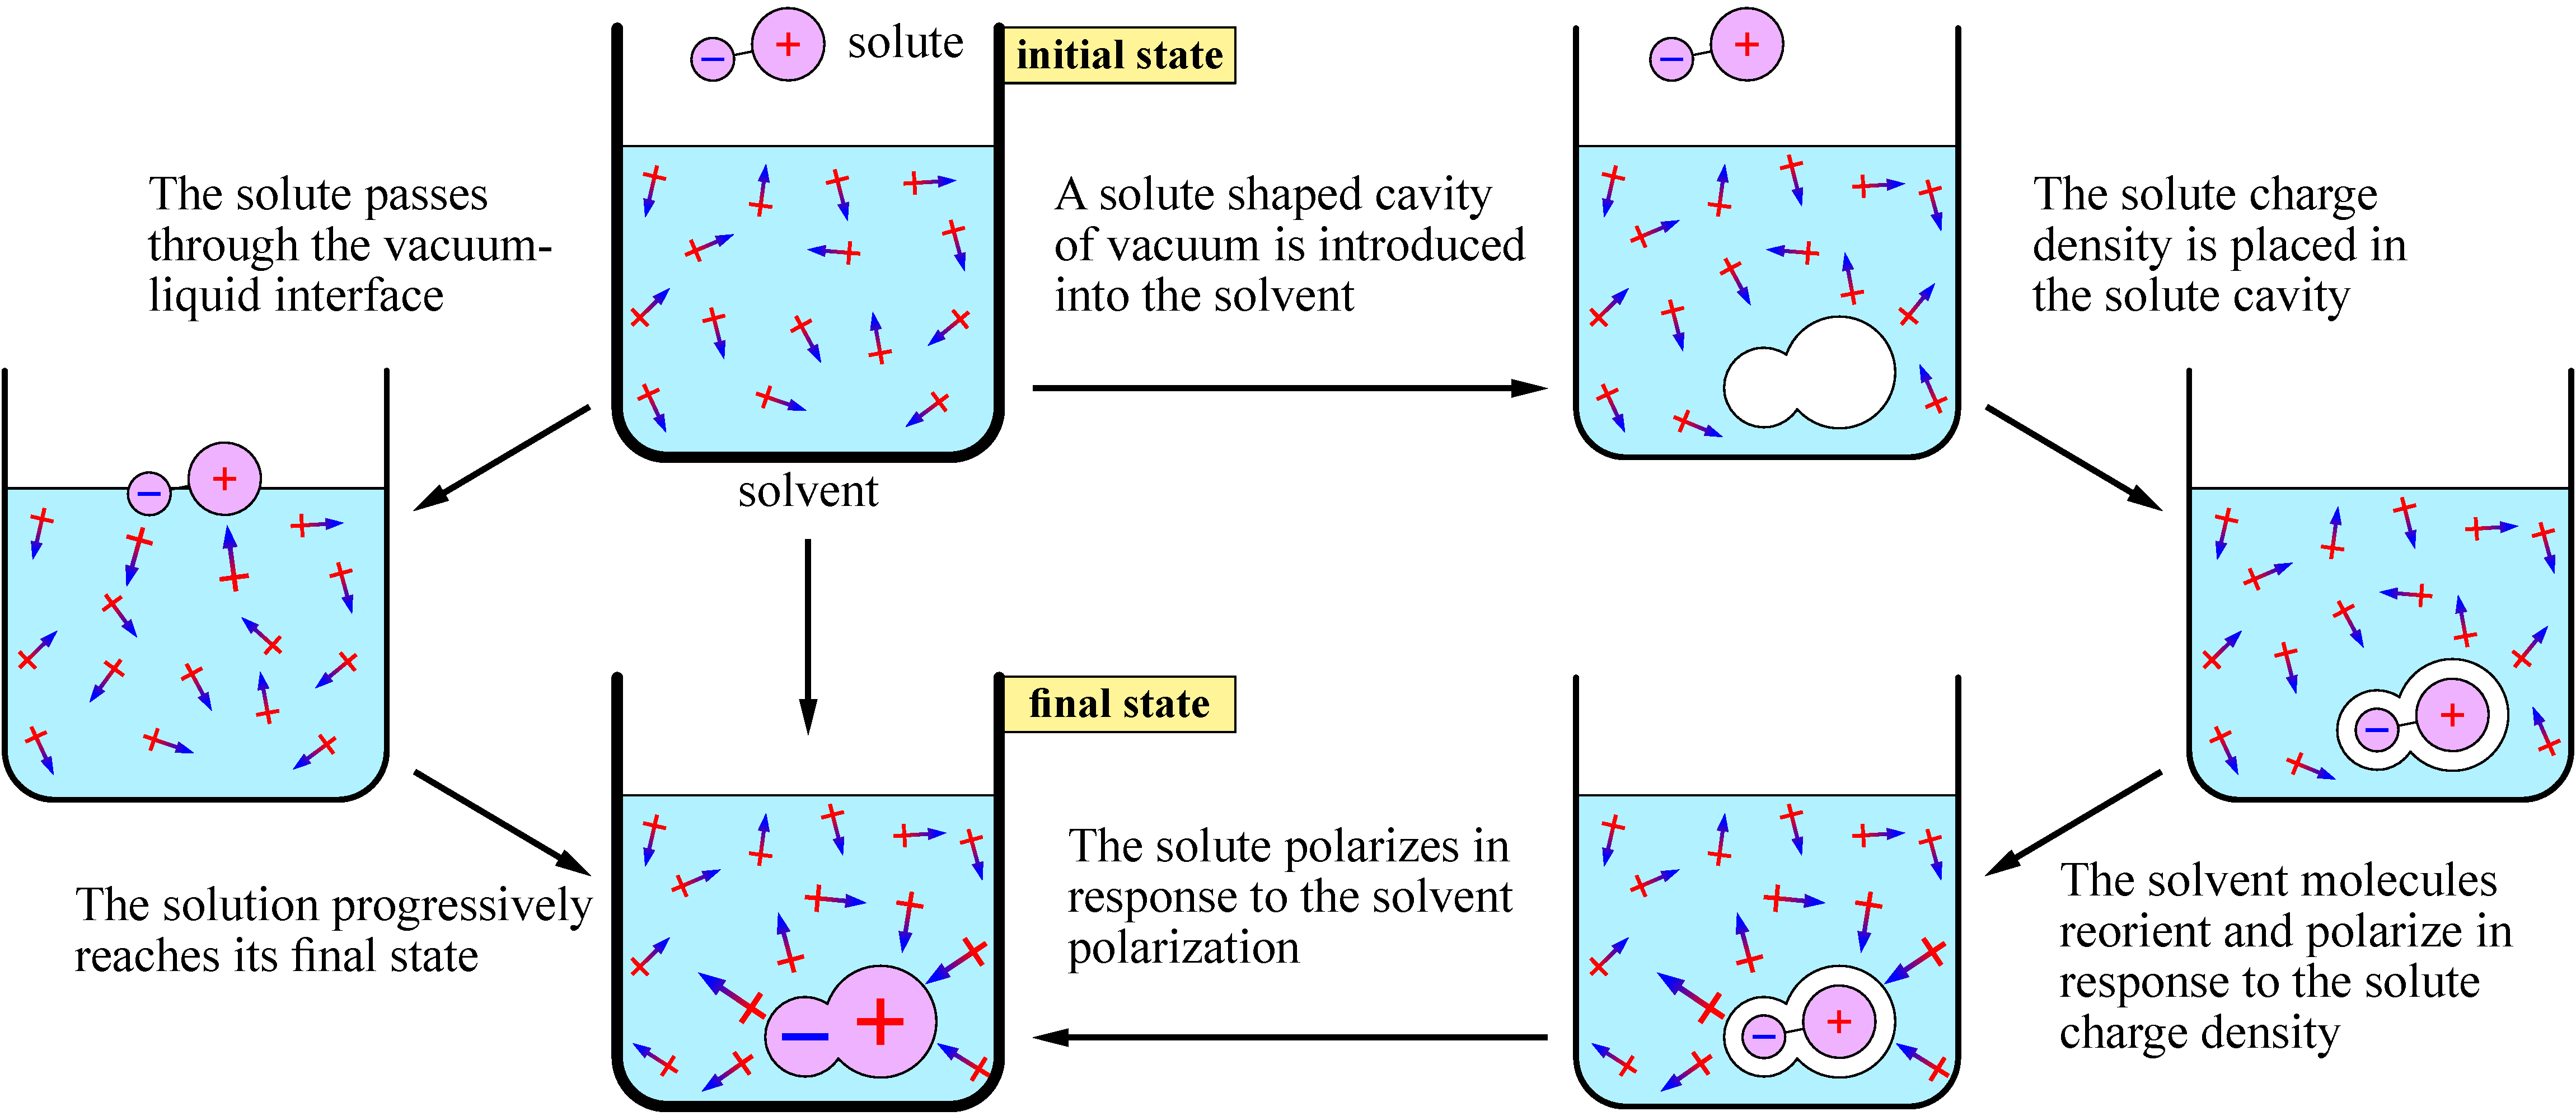
\includegraphics[width=1\columnwidth]{_figure/solvation}\caption[The solvation process]{The solvation process.\label{fig:Process-of-solvation} A thermodynamic
system, whose properties only depend on the initial and final states,
can go through different paths. The physical process of solvation
(left path) takes the solute from vacuum into bulk solvent, progressively
passing through the vacuum-liquid interface. Theoretically, the solvation
energy is defined as the energy consumed in such a process. In theoretical
studies, the process can be decomposed to some artificial unphysical
process (right path), involving the growth of an uncharged solute-sized
cavity within the bulk solvent, the transfer of the solute charge
distribution from vacuum into cavity, and the interaction between
the solute and solvent.}

\par\end{center}%
\end{minipage}
\end{figure}


As not all kinds of interactions are important in applications, different
models and methods have been developed according to the usage.

For most of the 20th century, the study of solvation effects has been
dominated by continuum (implicit) models \citep{Jensen,Cramer_1999},
which mostly rely on the continuum dielectric description of the solvent
and are not costly in terms of computation resources. They provide
an accurate way to treat the strong, long-range electrostatic interactions
which dominate many solvation phenomena, but lack detailed information
on the first solvation shell. This information mainly includes the
cavity formation energy and solute-solvent van der Waals interactions,
that are often rudely treated by introducing an artificial form of
cavity that links to the form of solute. The methods for testing electrostatic
interactions include the Generalized Born (GB) approximation or, for
better estimates, Poisson-Boltzmann (PB) calculations. These are widely
integrated within \acs{QM} simulations by adding extra solvation
terms onto the Fock or Kohn-Sham operator \citep{Tomasi_1994_implicit_model,tomasi_quantum_2005}.
However, the improper treatment of the first shell, where the microscopic
interactions are primarily located, often introduces potentially huge
errors in free energy evaluation, especially for polar solvents (such
as water), despite the accuracy that the \acs{QM} calculation alone
can achieve. Therefore, classical molecular simulations, which describe
the individual solvent molecules explicitly (explicit solvent), particularly
the molecular dynamics (\acs{MD}) and Monte Carlo method (\acs{MC}),
have become the alternative solution during the last few decades.
They generate trajectories and configurations, and from there estimate
free energy changes by statistical mechanical techniques, such as
free energy perturbation (FEP) theory or thermodynamic integration
(TI) \citep{Jorgensen_1995_MC}. These calculations are very demanding
in computing cost, due to the need for very many (hundreds or thousands)
solvent molecules to form a realistic model, and very many configurations
(millions) to be statistically significant.

Recently, a third domain of theory to describe solvents based on the
statistical mechanics of fluids has been growing rapidly. It mainly
involves the integral equation theory (\acs{IET}), and the classical
density functional theory (c\acs{DFT}) for liquids. These approaches
are capable of giving the molecular nature of the first solvation
shell, while without calculating all the instantaneous micro-states
with respect to time, but rather by integrating over positions and
momenta theoretically. Therefore, they are of orders of magnitude
faster than the simulations done by micro-states.

The integral equation theory (\acs{IET}) focuses on solving the Ornstein-Zernike
(\acs{OZ}) equation with a specific closure equation \citep{Hensen-McDonald,Gray-Gubbins}.
It was firstly limited to so-called ``simple liquids'' - a system
of spherical particles. The extension to molecular fluids, composed
of polyatomic molecules with non-spherical shapes, was done in two
different directions. On one hand, Chandler and Andersen in 1971 \citep{Chandler_1972_RISM}
developed the reference interaction site model (\acs{RISM}), which
discretizes the distribution and correlation functions into site-site
functions, and solves the \acs{OZ} equation and the closure in a
matrix \citep{hirata_molecular_2004}. On the other hand, Blum \citep{Blum_I,Blum_II},
Fries and Patey \citep{Fries_Patey_1985} extend the \acs{OZ} equation
into a full molecular form, where the distribution and correlation
functions depend on both position and orientation. In their theory,
the orientation part of \acs{OZ} equation is simplified by expanding
the distribution and correlation functions onto Wigner generalized
spherical harmonics.

The classical density functional theory approach deals with inhomogeneous
liquids, and uses the same variation principle and minimization strategy
\citep{mermin_thermal_1965,Evans_1979,Hansen_1987} as electronic
density functional theory (e\acs{DFT}) for electron-electron interactions.
The latter has received an immense success in computational chemistry.
Classical \acs{DFT} gives the Helmholtz free energy and the equilibrium
solvent density by minimizing the free energy functional of the solvent
density in the presence of a given external potential. Borgis and
collaborators \citep{gendre_classical_2009,jeanmairet_molecular_2013-1,jeanmairet_molecular_2015,jeanmairet_molecular_2016,Jeanmairet_thesis,levesque_solvation_2012,ramirez_density_2002,ramirez_density_2005,sergiievskyi_fast_2014,Zhao_2011}
have recently generalized it into the molecular case, leading to molecular
density functional theory (\acs{MDFT}), where the solvent density
depends on both position and orientation, $\rho(\mathbf{r},\mathbf{\Omega})$.
The main theoretical difficulty lies in the definition of well-funded
and reliable functionals of the excess free energy $\mathcal{F}_{\mathrm{exc}}\left[\rho\right]$,
accounting for the geometric complexity of the solvent molecule. Some
recent research has shown that \acs{MDFT} is capable to describe
linear solvents like acetonitrile, but but has still some caveats
for the most complex solvent, i. e. water \citep{Zhao_2011}. \acs{MDFT}
can be proven to be mathematically equivalent to the two-component
molecular \acs{IET}.

The majority of work of all these theories has been focused on water,
since it is one of the most difficult systems to model due to its
molecular geometry, unavoidable multi-body character, quantum effects,
and hydrogen bonds, etc. The importance of including instantaneous
polarization in potential functions is also an issue \citep{polarisable_1,polarisable_2}.
However, since polarizable force fields are not yet in common use,
the simulations by micro-states and the liquid theory which feed on
force fields also have their own limits, compared to the continuum
model which can be polarizable. The advantages and disadvantages of
each branch of theory are listed in table \ref{tab:Theories-of-solvation}.

\begin{table}[h]
\begin{centering}
\begin{tabular}{ccccc}
\toprule 
\tableheadline{Theory} & \tableheadline{Speed} & \tableheadline{Long-Range} & \tableheadline{First-Shell} & \tableheadline{Polarizable Solvent}\tabularnewline
\midrule
Continuum model & fast & yes & no & fully\tabularnewline
Simulation by time & costly & yes & yes & partially, very costly\tabularnewline
Theory of liquids & fast & yes & yes & partially\tabularnewline
\bottomrule
\end{tabular}
\par\end{centering}

\caption{Different solvation theories\label{tab:Theories-of-solvation}}
\end{table}



\section{Scope of this thesis}

This thesis aims to develop \acs{MDFT}, focusing on the generalization
and algorithmic acceleration of the excess free energy functional
$\mathcal{F}_{\mathrm{exc}}$ evaluation under homogenous reference
fluid (\acs{HRF}) approximation, which will be discussed in detail
in latter chapters. 

Chapter I reviews a selection of models and methods to describe solvent
effects. It includes the implicit and explicit models, the basics
of liquid-state theory, as well as its two frontier research domains,
\acs{IET} and \acs{MDFT}. The structure of the code named \acs{MDFT},
associated to the \acs{MDFT} approach, on which all the developments
of this thesis are based, is also presented. There is also a brief
introduction on how \acs{MD} and \acs{MC} simulations methods are
used to generate the direct correlation functions (\acs{DCF}) used
in this thesis.

Chapter II presents all the theory developed and newly used in this
thesis. Two algorithms for the excess energy functional evaluation
are proposed. One is an extension of the previous algorithm which
can be only applied to linear solvent, to a full 3D molecular solvent
case; while the other is a new algorithm, that combines the molecular
\acs{OZ} equation treatment of angular convolution with MDFT. The
solvation properties that the actual code generates are also presented,
mainly containing the free energy and solvent structure.

Chapter III reports all the implementation results, which are divided
into two aspects: the ``accuracy'', involves the error evaluations,
comparisons between algorithms and with \acs{IET} and \acs{MD} results;
and the ``efficiency'', evaluates the computing cost of the code,
of both in sequential and parallelized versions.

Chapter VI gives applications to ions and molecules. And some work
undone due to the limit of time are put in the perspective.
